\documentclass{article}

% Packages
\usepackage{amsmath} % For mathematical symbols and equations
\usepackage{graphicx} % For including images
\usepackage{cite} % For managing citations
\usepackage{lipsum} % For generating dummy text
\usepackage{algorithm} % For writing algorithms
\usepackage{algpseudocode} % For writing pseudocode
\usepackage{minted} % Syntax highlighting
\usepackage[a4paper, total={6in, 8in}]{geometry}
\usepackage{hyperref} % For hyperlinks

\title{Network Monitoring Report (PDSe)}
\author{Abhishta Gatya Adyatma}
\date{April 2024}

\begin{document}

\maketitle

\begin{figure}[htbp]
    \centering
    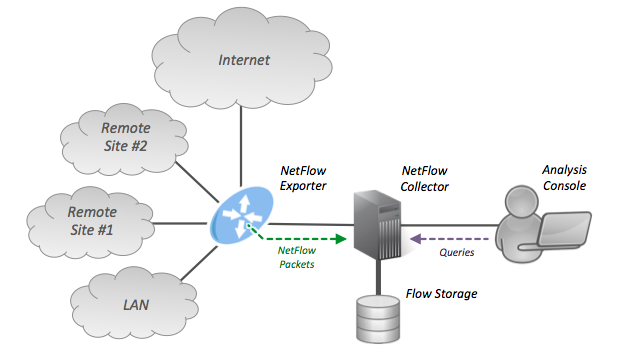
\includegraphics[width=0.6\linewidth]{img/NetFlow_Architecture_2012.png}
    \caption{NetFlow Architecture (wikipedia.org)}
    \label{fig:nfarch}
\end{figure}

\section{Introduction}

Network monitoring is the process of observing and analyzing the performance and behavior of computer networks. It ensures the smoothness of a network's operation, security, and efficiency through continuous surveillance of network devices, services, and traffic flows to detect issues. This report displays a network monitoring method through the NetFlow protocol for collecting IP traffic information and flow.

The NetFlow protocol is a network protocol developed by Cisco Systems that provides administrators visibility into the traffic flowing through their routers and switches. It works by capturing packets of information through NetFlow-capable devices as they pass through specific interfaces and identifying the packets' information such as their source, destination, protocol, etc. NetFlow also aggregates the data to provide details such as the number of packets, transmitted bytes, timestamps, and duration as it is being stored in a designated collector system as a flow record. The overview of the NetFlow protocol is illustrated through Figure \ref{fig:nfarch}.

This report documents the process of setting up a network monitoring system using NetFlow on the author's reported device with also an analysis of the captured data in various representations. The idea of the analysis is to explore the captured data and demonstrate how it can provide insight to network administrators. Exploration also includes discovering connections and the ability to explain them.

\section{Setup}

\begin{figure}[htbp]
    \centering
    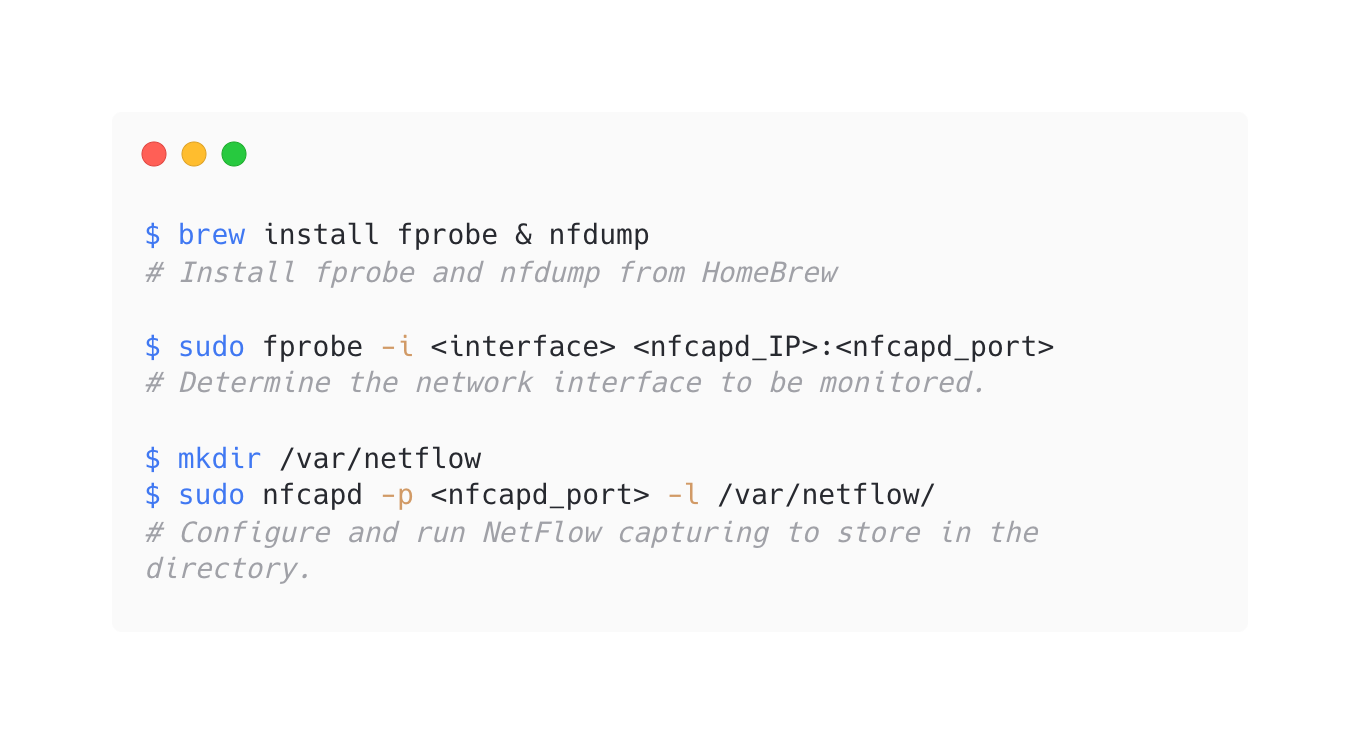
\includegraphics[trim=0 100 0 100,clip,width=1\linewidth]{img/nf-carbon.png}
    \caption{NetFlow Monitoring Setup}
    \label{fig:nfsetup}
\end{figure}

The author is using a MacBook Pro M1 with the Operating System of MacOS 14.4.1 and the M1 Architecture. With this, the author uses `fprobe` a tool used for collecting network traffic data and exporting it in the NetFlow format, and `nfcapd` a component of the NetFlow suite of tools used for collecting and storing NetFlow data. In summary, `fprobe` captures network traffic and generates NetFlow data, while `nfcapd` receives and stores the NetFlow data generated by probes like `fprobe`, making it available for analysis and monitoring. The setup process for this particular setup is visualized in Figure \ref{fig:nfsetup}.

\begin{figure}[H]
    \centering
    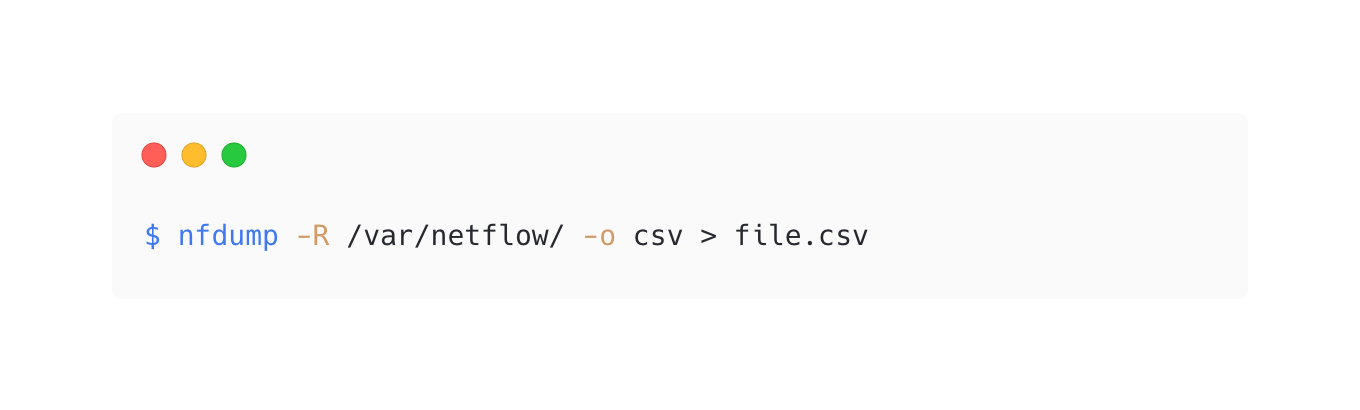
\includegraphics[trim=0 100 0 100,clip,width=1\linewidth]{img/nfd-carbon.png}
    \caption{NetFlow Dump as CSV}
    \label{fig:nfdump}
\end{figure}

The data collected using the NetFlow protocol is stored in binary format for processing efficiency and performance. However, the author prefers to extract the data into a CSV (Comma Separated Value) format that is easier to process with various Python libraries such as NumPy and Pandas. Therefore, the process of extracting the NetFlow binary into a CSV format is visualized in Figure \ref{fig:nfdump}.

\section{Analysis}

This section covers the basic analysis of the captured NetFlow data over 56+ Hours (over 4 days of usage). After removing bad data (flows of duration value 0 and null values), it captures a collected size of 96 MB of 783,813 flows spanning 438,283 unique connections and 9,657 IPs. The author has collected over 4.6 GB and 10,770,951 Packets of Transmission.

\subsection{Captured Protocol (\%)}

\begin{figure}[htbp]
    \centering
    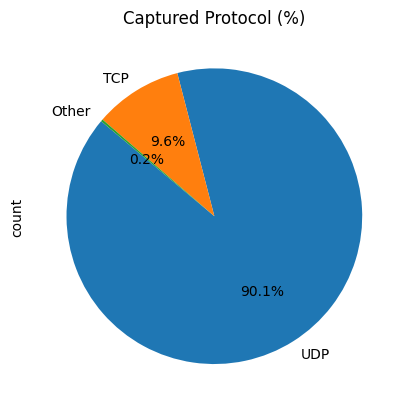
\includegraphics[width=0.4\linewidth]{img/capp.png}
    \caption{Percentage of Captured Flows Protocols}
    \label{fig:nfanalcap}
\end{figure}

Figure \ref{fig:nfanalcap} shows that out of the 1,337,158 flows decompose to 90.1\% UDP, 9.6\% TCP, and 0.2\% Other (IGMP, ICMP, IPv6, etc.) Traffic. This is to be expected since many network protocols and applications use UDP for their communication due to its lower latency, better performance, and lightweight nature compared to TCP. This preference for UDP makes it frequent in network traffic and thus prominent in NetFlow data captures. In further investigation, the author will display a representation of separated traffic by UDP and TCP.

\subsection{Bytes, Packets \& Flows in Periodic Traffic}

\begin{figure}[htbp]
    \centering
    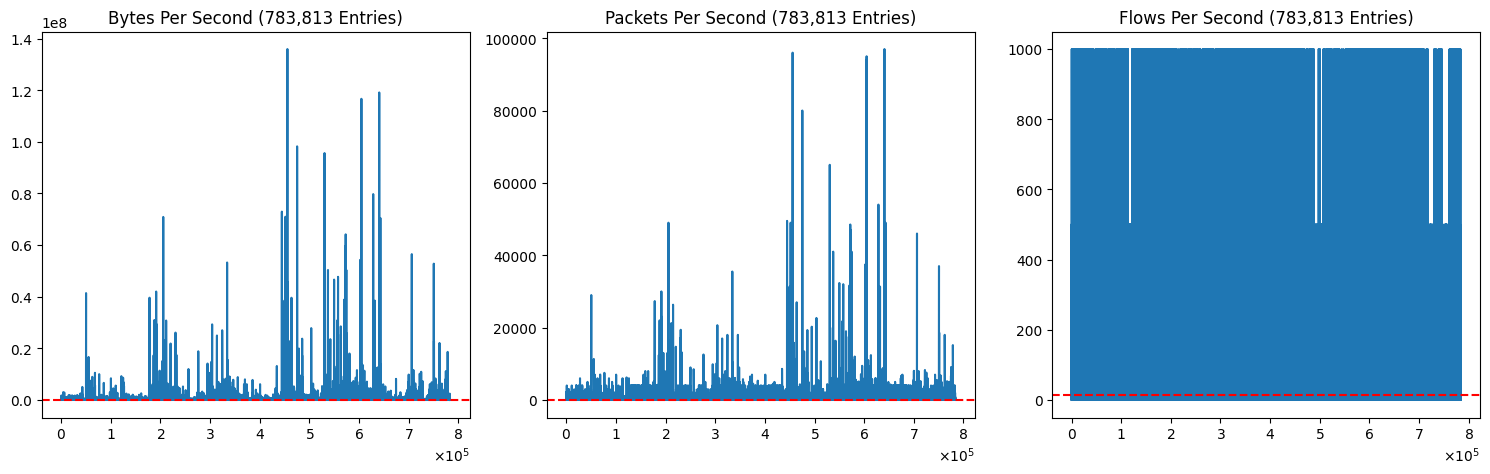
\includegraphics[width=1\linewidth]{img/bpf-all.png}
    \caption{Bytes, Packets, \& Flows of All Traffic}
    \label{fig:nfanalbpf}
\end{figure}

Figure \ref{fig:nfanalbpf} shows the Bytes, Packets, and Flows per Second of all 56+ Hours of traffic. However, this visualization is not quite intelligible to understand the network's overall performance fluctuation due to the sheer high volume of data. This data would not provide insight to network administrators. In light of this, the author decides to average the statistics hourly to get an aggregation of the hourly Bytes-per-second (BPS), Packets-per-second (PPS), and Flows-per-seconds (FPS).

\begin{figure}[htbp]
    \centering
    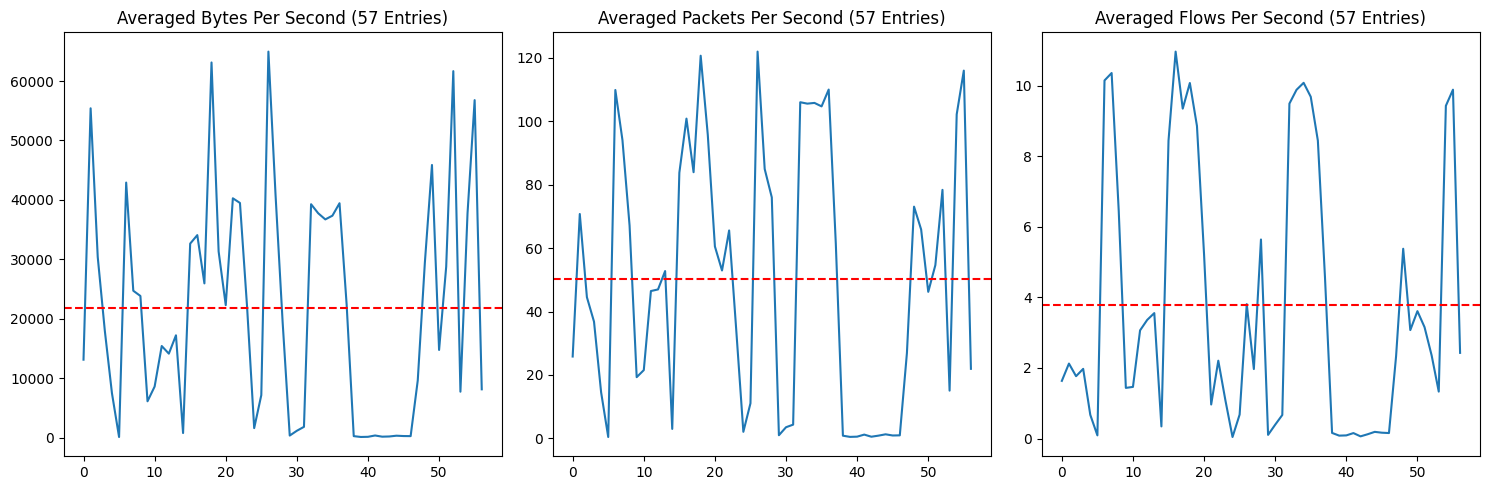
\includegraphics[width=1\linewidth]{img/bpf-h.png}
    \caption{Averaged Hourly Bytes, Packets, \& Flows of All Traffic}
    \label{fig:nfanalbpfh}
\end{figure}

Figure \ref{fig:nfanalbpfh} improves clarity over the volume of data, capturing the hourly BPS, PPS, and FPS in order. The figure shows the peaks and valleys displaying the most active hours and idle hours (over 4 days of usage). It is interesting that the idle use of this device (shown in the range of 40 - 50) still communicates with some connection even though the device is not in use (in sleep mode). Further, the author displays the BPS, PPS, and FPS separated by the TCP and UDP protocols.

\begin{figure}[htbp]
    \centering
    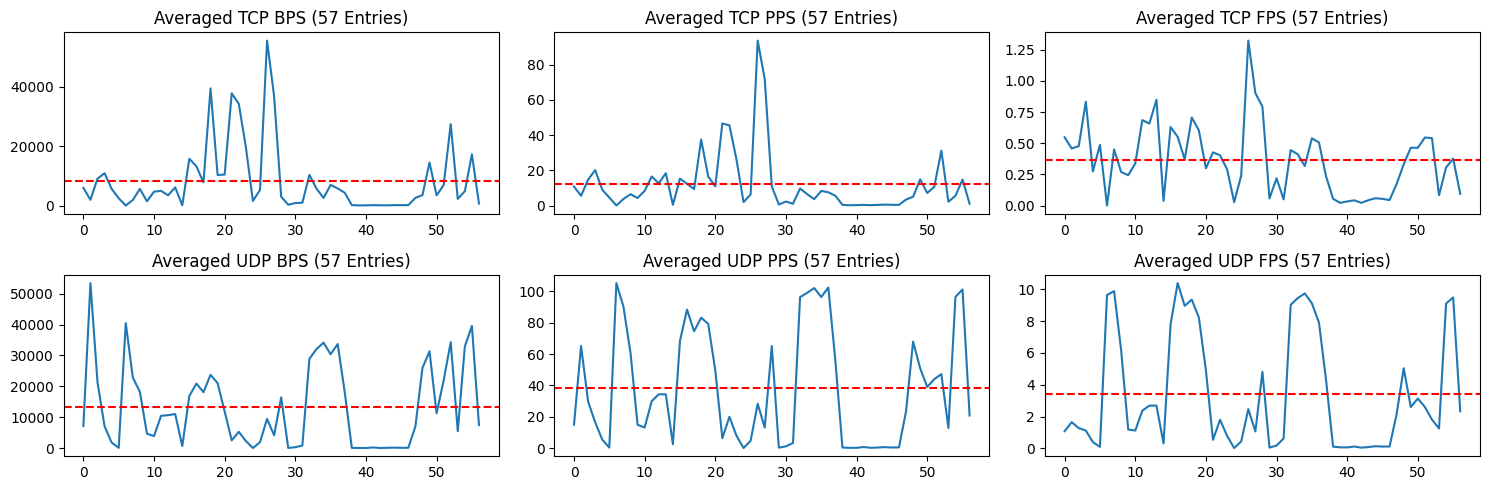
\includegraphics[width=1\linewidth]{img/bpf-h-s.png}
    \caption{Averaged Hourly Bytes, Packets, \& Flows of Traffic by Protocol (TCP \& UDP)}
    \label{fig:nfanalbpfhs}
\end{figure}

Figure \ref{fig:nfanalbpfh} separates the traffic by protocol and displays the averaged hourly BPS, PPS, and FPS of the collected data. Deconstructing the BPS, PPS, and FPS further improves clarity in understanding the protocol usage of the collected data and here it displays that some peaks and valleys are not aligned with each other. Furthermore, the author explores the connections associated with the traffic to understand the most frequent sites that the author potentially visits (knowingly or unknowingly).

\subsection{Frequent Sites by Bytes \& Packets}

\begin{table}[H]
    \centering
    \begin{tabular}{ccc}
         Rank. & Site (TLD) & Transmitted Bytes (MB)\\
         \hline
         1. & vutbr.cz & 966.9 MB \\
         2. & 1e100.net & 403.5 MB \\
         3. & akamaitechnologies.com & 89.6 MB \\
         4. & googleusercontent.com & 58.8 MB \\
         5. & cloudfront.net & 34.9 MB \\
         6. & amazonaws.com & 16.7 MB \\
         7. & github.com & 16.2 MB \\
         8. & yahoo.com & 5.6 MB \\
         9. & aaplimg.com & 5.5 MB \\
         10. & fbcdn.com & 3 MB \\
    \end{tabular}
    \caption{Most Frequent Sites by Total Transmitted Bytes}
    \label{tab:nfsite-bytes}
\end{table}

\begin{table}[H]
    \centering
    \begin{tabular}{ccc}
         Rank. & Site (TLD) & Transmitted Packets\\
         \hline
         1. & vutbr.cz & 5,094,649 \\
         2. & 1e100.net & 552,713 \\
         3. & googleusercontent.com & 242,745 \\
         4. & amazonaws.com & 101,704 \\
         5. & cloudfront.net & 93,256 \\
         6. & akamaitechnologies.com & 82,407 \\
         7. & github.com & 36,512 \\
         8. & yahoo.com & 14,782 \\
         9. & facebook.com & 8,190 \\
         10. & aaplimg.com & 6,541 \\
    \end{tabular}
    \caption{Most Frequent Sites by Total Transmitted Packets}
    \label{tab:nfsite-packets}
\end{table}

Aggregating the most frequent sites requires the author to get the site information from IPs automatically. Using Python's `socket.gethostbyaddr(ip)` function was sufficient for this particular task to get the Top Level Domain (TLD). However, the function requires a connection to be established to retrieve the desired information. The connection can be an unreliable variable as it relies on the performance and reachability of the site. If a site is unreachable, it waits until a Time Out which is not ideal.

To mitigate potential Time Out and the consequential slowdown of this process, the author identifies the source of the IPs that cause it. The author finds that Lower-rank IPs (in terms of their Total Bytes / Packets Transmitted) are the most likely to cause a slowdown due to unreachability. With this intuition, the author searches for an optimal threshold that was able to split the data into Upper Bounds and Lower Bounds having the Upper Bound Rank best describing the whole captured data to find the most frequent sites with an accurate approximation of Total Transmitted Bytes / Packets. For estimating the most frequent sites with Total Bytes Transmitted, a threshold of 0.65 MB found that the Upper Bound was able to describe 83\% of the data with only 983 IPs, and estimating the most frequent sites with Total Packets Transmitted used a threshold of 1000 Packets to describe 82\% of the data with only 2125 IPs.

Table \ref{tab:nfsite-bytes} and \ref{tab:nfsite-packets} displays the top 10 most frequent sites by Total of Transmitted Bytes and Packets by the author. While the domain `vutbr.cz` is to be expected, the domain `1e100.net` strikes out as a domain that the author is unfamiliar with. Through some research, it seems it's owned by Google to identify our servers across all Google products (\url{https://support.google.com/faqs/answer/174717?hl=en}). Furthermore, interestingly the ranks for Total Transmitted Bytes and Packets differ slightly as some site sends more Bytes than Packets and vice versa.

\subsection{Frequent Autonomous System Destination by Bytes \& Packets}

\begin{table}[H]
    \centering
    \begin{tabular}{cccc}
         Rank. & AS Number & AS Description & Transmitted Bytes (MB)\\
         \hline
         1. & 13335 & CLOUDFLARENET, US & 1,010.3 MB \\
         2. & 714 & APPLE-ENGINEERING, US & 781.3 MB \\
         3. & 15169 & GOOGLE, US & 428.7 MB \\
         4. & 197451 & VUTBR-AS, CZ & 209.2 MB \\
         5. & 201263 & AS-BRIX-CDN, CZ & 183 MB \\
         6. & 15133 & EDGECAST, US & 139.5 MB \\
         7. & 54113 & FASTLY, US & 69.5 MB \\
         8. & 16509 & AMAZON-02, US & 28.9 MB \\
         9. & 13414 & TWITTER, US & 22.2 MB \\
         10. & 396982 & GOOGLE-CLOUD-PLATFORM, US & 16.0 MB \\
    \end{tabular}
    \caption{Most Frequent Autonomous Systems by Total Transmitted Bytes}
    \label{tab:nfas-bytes}
\end{table}

\begin{table}[H]
    \centering
    \begin{tabular}{cccc}
         Rank. & AS Number & AS Description & Transmitted Packets\\
         \hline
         1. & 197451 & VUTBR-AS, CZ & 1,197,469 \\
         2. & 714 & APPLE-ENGINEERING, US & 1,145,514 \\
         3. & 13335 & CLOUDFLARENET, US & 1,009,817 \\
         4. & 15169 & GOOGLE, US & 612,080 \\
         5. & 201263 & AS-BRIX-CDN, CZ & 166,998 \\
         6. & 15133 & EDGECAST, US & 114,095 \\
         7. & 14618 & AMAZON-AES, US & 97,604 \\
         8. & 16509 & AMAZON-02, US & 96,093 \\
         9. & 54113 & FASTLY, US & 64,376 \\
         10. & 13414 & TWITTER, US & 50,981 \\
    \end{tabular}
    \caption{Most Frequent Autonomous Systems by Total Transmitted Packets}
    \label{tab:nfas-packets}
\end{table}

Aggregating the most frequent autonomous system (AS) destination requires the author to get deeper information from IPs automatically. This can be done through a WHOIS Lookup which is a query and response protocol that is used for querying databases that store an Internet resource's registered users or assignees. This information is maintained by the Internet Assigned Numbers Authority (IANA) an organization that oversees global IP addresses and stores information regarding Autonomous Systems (AS), Associated Organizations, Network Range, etc. Using a Python library called `ipwhois`, the author was able to automate this process and apply the same intuition that is used to gather the site information to significantly lower the number of searches to approximate the most frequent AS destinations.

Table \ref{tab:nfas-bytes} and \ref{tab:nfas-packets} displays the top 10 most frequent AS destinations by Total of Transmitted Bytes and Packets by the author. Claiming the top position seems to be clear as CloudFlare is a Content-Delivery Network (CDN) that is used for multiple visited sites and stores their resources within the network. Apple Engineering is expected as well as any Apple ecosystem will connect to Apple services such as iCloud, iMessage, Apple Music, etc. This goes without saying that different devices will most likely connect to their ecosystem of services that will claim the top ranks within AS destinations.

\subsection{Port Usage Frequency in Traffic}

\begin{table}[H]
    \centering
    \begin{tabular}{ccccc}
         Rank. & Port & Protocol & Frequency & Description \\
         \hline
         1. & 5353 & UDP & 479,346 & Multicast DNS (mDNS)\\
         2. & 1900 & UDP & 386,324 & Simple Service Discovery Protocol (SSDP) \\
         3. & 443 & TCP & 93,536 & HTTPS / SSL\\
         4. & 3702 & TCP/UDP & 23,769 & Web Service Discovery (WSD) \\
         5. & 137 & UDP & 16,580 & Windows Internet Naming Service (WINS) \\
         6. & 138 & UDP & 6,662 & NETBIOS Datagram Service \\
         7. & 57621 & UDP & 5,184 &  Spotify Client for P2P Communication \\
         8. & 17500 & TCP/UDP & 4,730 & Dropbox LanSync Protocol \\
         9. & 0 & - & 3,172 & System Reserved \\
         10. & 22222 & UDP & 2,477 & System Reserved \\
    \end{tabular}
    \caption{Port Usage Frequency in Traffic with Description}
    \label{tab:nfport}
\end{table}

Table \ref{tab:nfport} examines the usage frequency of ports within the traffic as part of the analysis. Well-known ports of the range 0 - 1024 are surprisingly not quite that prevalent within the traffic captured. However, as expected the mDNS and SSDP ports claim the top positions of usage as mDNS is a protocol used on local networks for resolving hostnames and SSDP is a protocol used for service discovery and announcement within a local network environment. Interestingly, the captured data also shows a user application client using port 57621 using the UDP protocol. This data can also be used for security examination of identifying malicious applications attempting to use a seemingly foreign port or disguising it as a proper service port.

\section{Conclusion}

NetFlow is a powerful network protocol capable of efficiently collecting and aggregating data, offering valuable insights for network administrators and researchers. Effective monitoring and analysis of this data is crucial for ensuring the smooth operation, security, and optimization of modern computer networks. Furthermore, network analysis holds valuable insights for capacity planning and resource allocation, empowering organizations to optimize their network infrastructure and resource utilization. This project serves as a demonstration of the potential of network protocols in gathering data and understanding device usage patterns. Leveraging NetFlow data opens doors to conducting multiple other analyses, from forecasting future traffic trends to geolocating traffic destinations by AS, unlocking deeper insights for informed decision-making and proactive network management.

\end{document}
